\chapter{Experimental}
\label{ch:chap05}

\section{Ambiente de prueba}
\label{sec:hardware}

\begin{table}[H]
	\begin{tabular}{ll}
		Procesador & Intel i7 8700K - 12 CPUs - 3.7 GHz       \\\cline{1-1}
		GPU        & Nvidia GeForce GTX 1070 Ti - 8 GiB  VRAM \\\cline{1-1}
		RAM        & 32 GiB - 2667 MHz                        \\\cline{1-1}
	\end{tabular}
	\caption{Características del hardware utilizado}
\end{table}

\begin{table}[H]
	\begin{tabular}{ll}
		SO & Windows 10 Pro       \\\cline{1-1}
		Embree        & v3.5.2  \\\cline{1-1}
		OpenGL        & v4.5                        \\\cline{1-1}
	\end{tabular}
	\caption{Características del software utilizado}
\end{table}

\begin{tabular}{@{} *5l @{}}    \toprule
	\textit{name} & \textit{foo} &&&  \\\midrule
	Models    & A  & B  & C  & D  \\ 
	Model $X$ & X1 & X2 & X3 & X4\\ 
	Model $Y$ & Y1 & Y2 & Y3 & Y4\\\bottomrule
	\hline
\end{tabular}
\section{Escenas}
\label{sec:escenas}

Con el objetivo de obtener resultados comparables para los distintos algoritmos y configuraciones se plantea el uso de dos escenas particulares de prueba, con distintas variaciones en los materiales que componen cada una de ellas.



Se denominará \textit{Escena - Conrnell Box} a la referente a la figura \ref{img:cornell}. Se basa en un tipo de escena comúnmente usado en el se ubican objetos en el interior de una caja (cubo) donde debajo están los objetos de prueba y en el nivel superior reside el objeto que emitirá luz. Esta escena cuenta con siete objetos, el cubo, una esfera que oficia de luz, y cinco objetos compuestos por diversas primitivas. En total, existen 12.922 caras de las cuales 96 son triangulares y 12.826 son cuadrilaterales. Cabe notar, que de haber soportado únicamente caras triangulares se procesarían 25.748 parches.

\begin{figure}[H]
	\centering
	\begin{subfigure}{0.45\textwidth}
		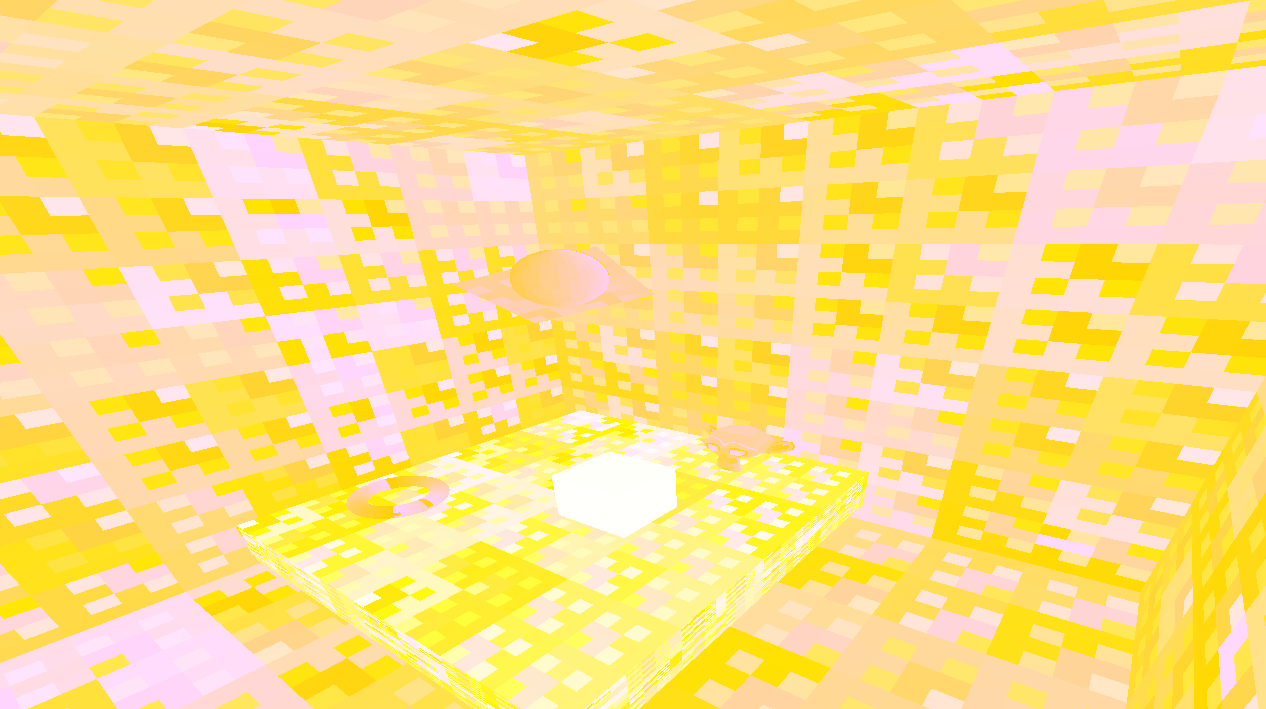
\includegraphics[width=1\linewidth]{assets/cornell}
		\caption{Vista lateral}
	\end{subfigure}
	\begin{subfigure}{0.45\textwidth}
		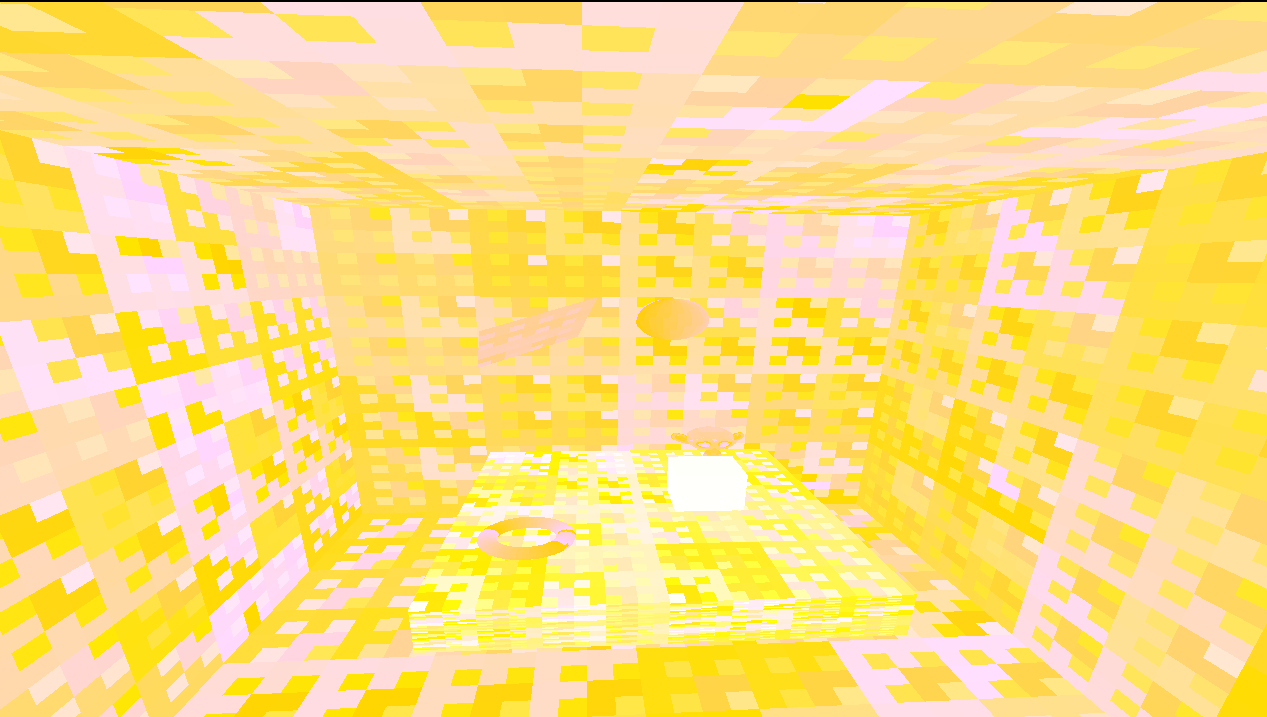
\includegraphics[width=1\linewidth]{assets/cornell2}
		\caption{Vista frontal}
	\end{subfigure}
	\caption{Vistas de la escena \textit{Conrnell Box}}
	\label{img:cornell}
\end{figure}

Se denominará \textit{Escena - Calle} a la referente a la figura \ref{img:street}. La escena está construida por dos objetos, el primero de ellos es una cúpula (hemi-esfera) subdividia en 2.407 cuadriláteros de área equitativa, su objetivo es representar el cielo. Por otro lado, el segundo objeto es una representación de ... . En total, las escena cuenta con 61.795 caras cuadrilaterales.

\begin{figure}[H]
	\centering
	\begin{subfigure}{0.45\textwidth}
		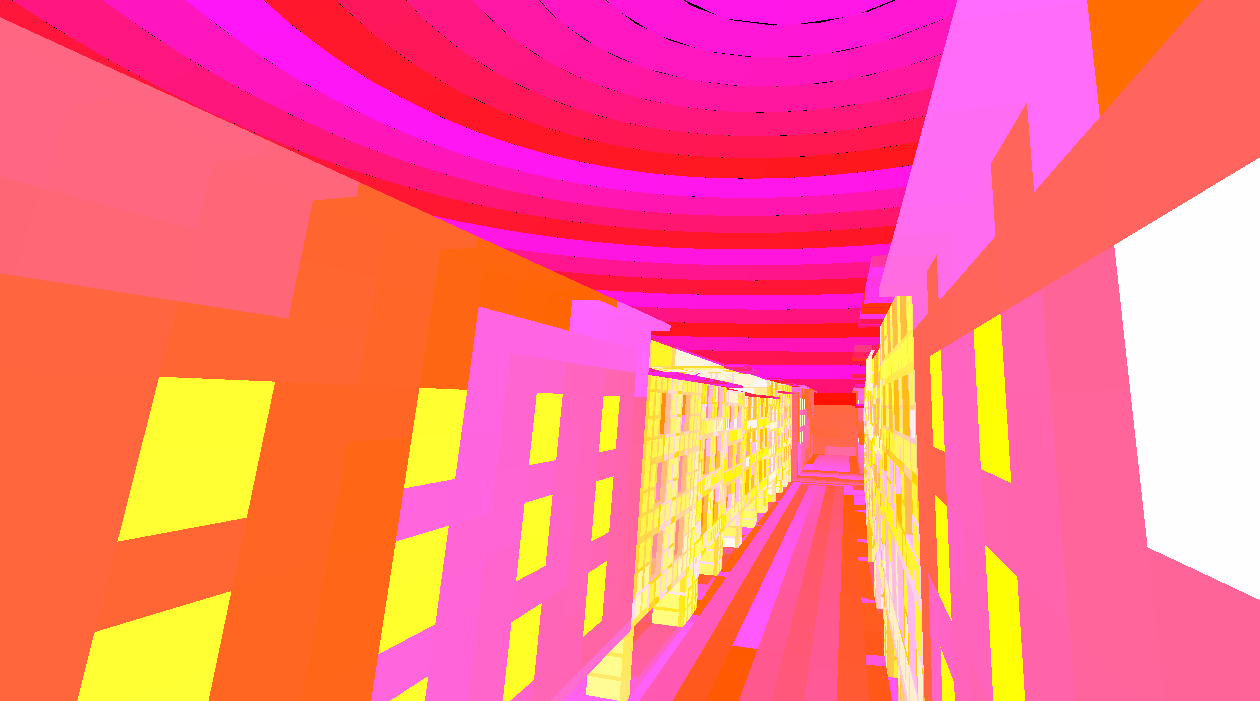
\includegraphics[width=1\linewidth]{assets/street1}
		\caption{Vista desde la ventana de una de las edificaciones}
	\end{subfigure}
	\begin{subfigure}{0.45\textwidth}
	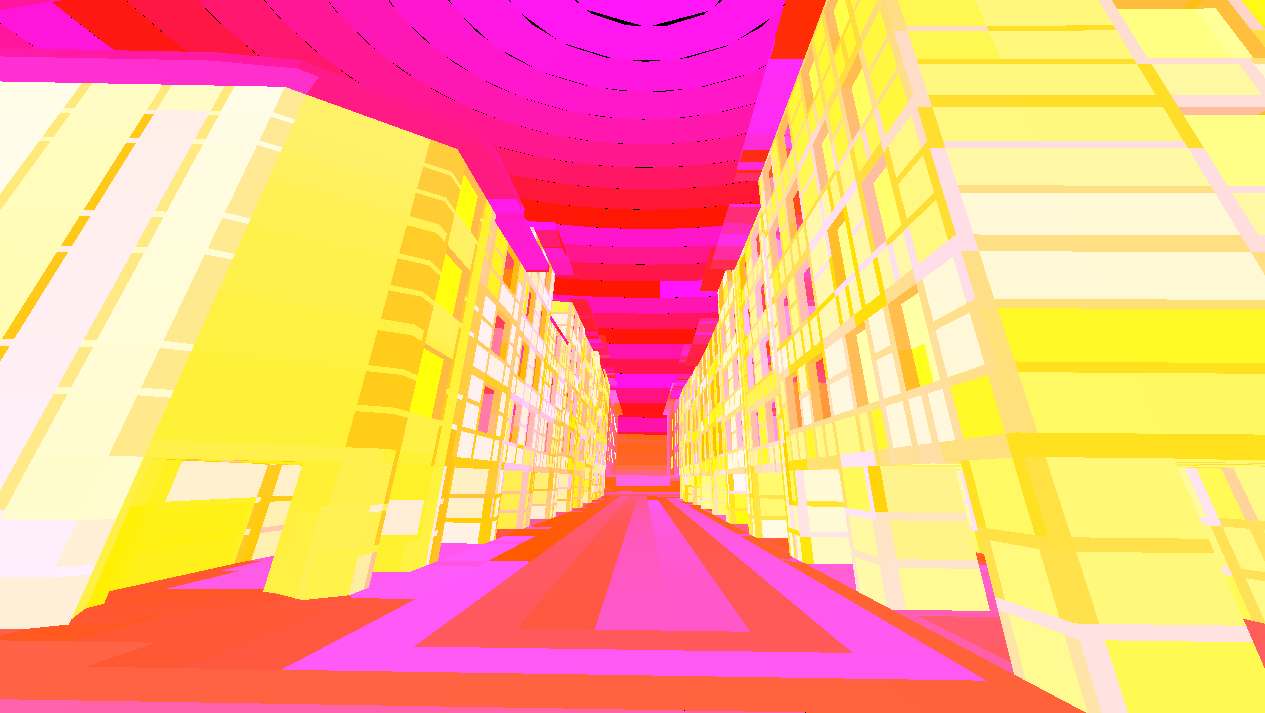
\includegraphics[width=1\linewidth]{assets/street2}
	\caption{Vista desde uno de los extremos de la calle}
	\end{subfigure}
	\begin{subfigure}{0.45\textwidth}
	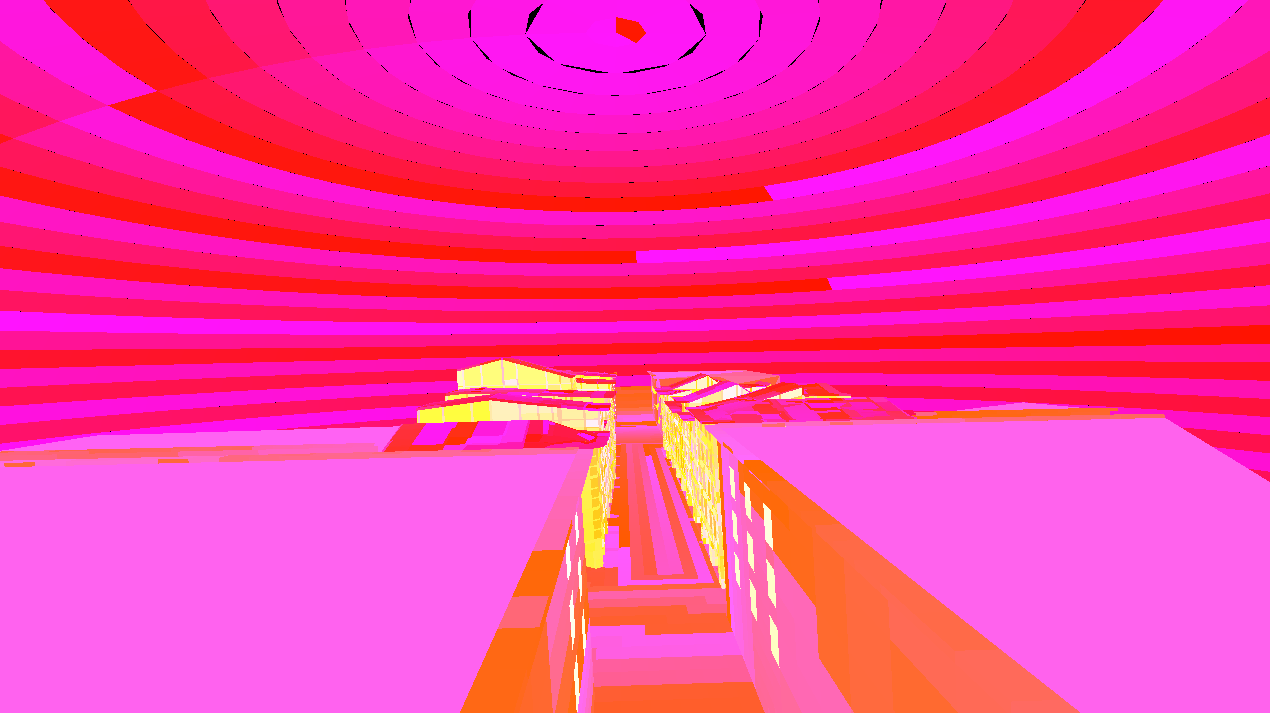
\includegraphics[width=1\linewidth]{assets/street3}
	\caption{Vista aérea}
	\end{subfigure}
	\begin{subfigure}{0.45\textwidth}
	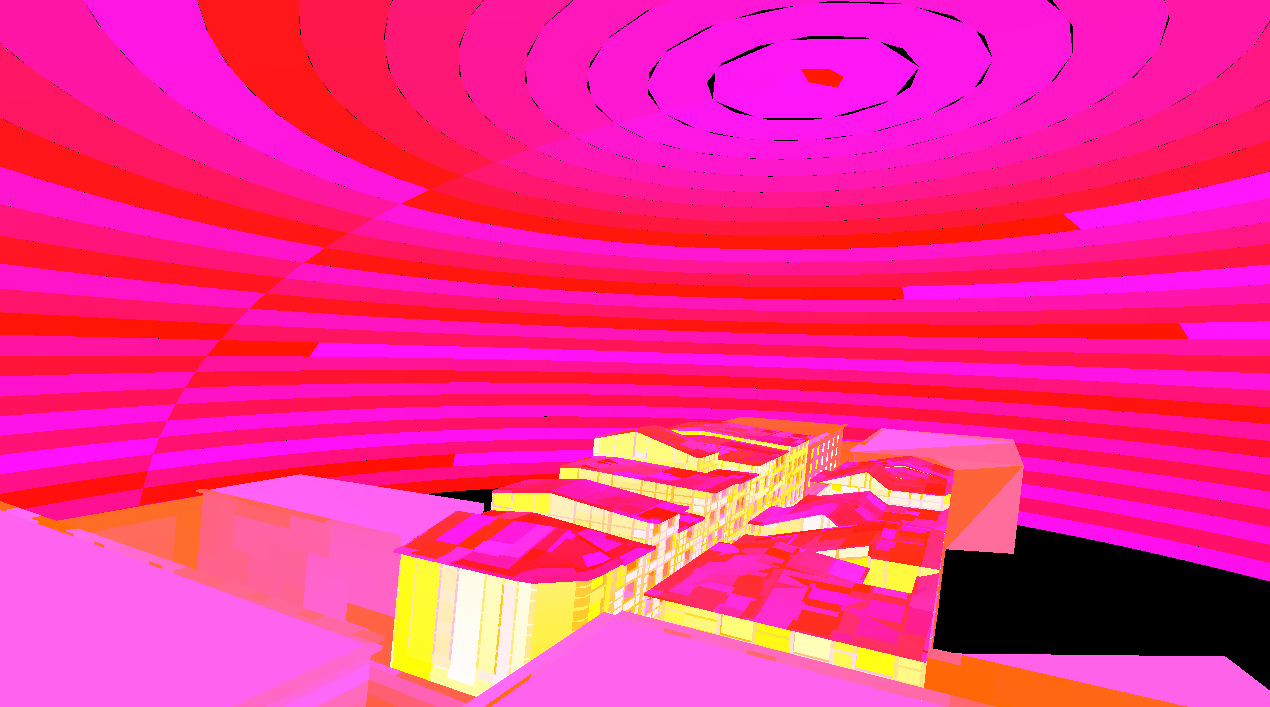
\includegraphics[width=1\linewidth]{assets/street4}
	\caption{Vista aérea}
	\end{subfigure}
	\caption{Vistas de la escena \textit{Calle}}
	\label{img:street}
\end{figure}
\section{Casos de prueba}
\label{sec:pruebas}

Se proponen casos de prueba utilizando las escenas descritas en \ref{sec:escenas} utilizando diversos materiales.

\subsection{Métricas consideradas}

Con el objetivo de medir correctamente las ventajas y desventajas de cara acercamiento al cálculo de factores de forma simples y extendidos que se han propuesto, se definirán un conjunto de métricas para evaluar su optimialidad en distintas dimensiones.

\begin{itemize}
	\item Dimensión rendimiento
		\begin{itemize}
			\item Tiempo de ejecución: Se registrará el tiempo empleado en calcular completamente la matriz de factores de forma.
		\end{itemize}
	\item Dimensión matriz de factores de forma: Se computará la matriz de factores de forma de control $\mathbf{F_{C}}$ utilizando la técnica de trazado de rayos con una gran resolución.
		\begin{itemize}
			\item Error promedio de factor de forma por fila: $Ep_{i} = \sum_{j=1}^{N} \frac{|\mathbf{F}_{ij} -\mathbf{F}_{ij}|}{N}$
			\item Error máximo de factor de forma por fila: $Em_{i} = \max_{j=1}^{N}|\mathbf{F}_{ij} -\mathbf{F}_{ij}|$
			\item Error estándar de factor de forma por fila: $Em_{i} = \max_{j=1}^{N}(\mathbf{F}_{ij} -\mathbf{F_{C}}_{ij})^{2}$
		\end{itemize}
	\item Dimensión vector de radiosidad:
	\begin{itemize}
		\item Error promedio de radiosidad: $Ep = \sum_{i=1}^{N} \frac{|R_{i}-R_{Ci}|}{N}$
		\item Error máximo de radiosidad
		\item Error estándar de radiosidad
	\end{itemize}
\item Dimensión visual:
	\begin{itemize}
		\item Calidad de resultados
	\end{itemize}
\end{itemize}
